\documentclass[a4paper,11pt]{article}
\usepackage[utf8]{inputenc}
\usepackage{minted}
\usepackage{amsmath}
\usepackage{float}
\usepackage{graphicx}
\usepackage[toc,page]{appendix}

\graphicspath{{./figures/}}

\title{\textbf{2. Sorted arrays}}
\author{Kristiāns Vinters}
\date{Fall 2023}

\begin{document}
    \maketitle
    \section*{Introduction}

    I solved the sorted array search assignment in Go. I used Go because I want to become more familiar with it. Source code and benchmark data is available on GitHub\footnote{https://github.com/Phanty133/id1021/tree/master/2-sorted}.

    \section*{Implementation}

    I implemented all of the search and duplicate functions using generic typing with the constraint \texttt{cmp.Ordered}, which constrains the type to anything that implements the \texttt{==}, \texttt{!=}, \texttt{<}, \texttt{>}, \texttt{>=}, \texttt{<=} operators. Frankly, there is no particular reason to do so for this assignment other than to get more familiar with Go's generics.

    There weren't any particular difficulties in implementing the search and duplicate functions in Go. The implementations for the unordered, ordered, and binary search closely follow the given example Java implementations.

    \begin{figure}[H]
        \centering
        \begin{minted}{go}
func NaiveSearch[T cmp.Ordered](arr []T, target T) int {
    for i := 0; i < len(arr); i++ {
        if arr[i] == target {
            return i
        }
    }

    return -1
}
        \end{minted}
        \caption{Naive search implementation}
        \label{fig:naive-search}
    \end{figure}

    \begin{figure}[H]
        \centering
        \begin{minted}{go}
func NaiveSortedSearch[T cmp.Ordered](arr []T, target T) int {
    for i := 0; i < len(arr); i++ {
        if arr[i] > target {
            return -1
        }

        if arr[i] == target {
            return i
        }
    }

    return -1
}
        \end{minted}
        \caption{Naive sorted search implementation}
        \label{fig:naive-sorted-search}
    \end{figure}

    \begin{figure}[H]
        \centering
        \begin{minted}{go}
func BinarySearch[T cmp.Ordered](arr []T, target T) int {
    first := 0
    last := len(arr) - 1

    for {
        idx := (first + last) / 2
        val := arr[idx]

        if val == target {
            return idx
        }

        if val < target && idx < last {
            first = idx + 1
        } else if val > target && idx > first {
            last = idx - 1
        } else {
            return -1
        }
    }
}
        \end{minted}
        \caption{Binary search implementation}
        \label{fig:binary-search}
    \end{figure}

    The duplicate finding functions were also straightforward to implement and two of the three utilized the search functions. The \texttt{DuplicatesNaive} and \texttt{DuplicatesBinary} were implemented almost exactly the same apart from using different search functions.

    \begin{figure}[H]
        \centering
        \begin{minted}{go}
// or DuplicatesBinary[T cmp.Ordered](a []T, b []T) []T
func DuplicatesNaive[T cmp.Ordered](a []T, b []T) []T {
    res := make([]T, 0, len(a)+len(b))

    for _, v := range a {
        // or if BinarySearch(b, v) != -1 {
        if NaiveSearch(b, v) != -1 {
            res = append(res, v)
        }
    }

    return res
}
        \end{minted}
        \caption{Naive and binary duplicate finding implementation}
        \label{fig:duplicates}
    \end{figure}

    The final duplicates function, \texttt{SortedDuplicatesSmart}, didn't use any of the search functions, but rather iterated over both array's indices simultaneously.

    \begin{figure}[H]
        \centering
        \begin{minted}{go}
func SortedDuplicatesSmart[T cmp.Ordered](a []T, b []T) []T {
    res := make([]T, 0, len(a)+len(b))

    i := 0
    j := 0

    for i < len(a) && j < len(b) {
        if a[i] > b[j] {
            j++
        } else if a[i] < b[j] {
            i++
        } else {
            res = append(res, a[i])
            i++
            j++
        }
    }

    return res
}
        \end{minted}
        \caption{Smart duplicate finding implementation}
        \label{fig:smart-duplicates}
    \end{figure}

    \section*{Benchmarking}

    To benchmark the functions, I rewrote the given example benchmarking function given in \texttt{Bench.java} to Go as the \texttt{bench} package. The Go implementation improves upon the example by making the benchmarkable function as a function argument and also determining median and mean times, in addition to min and max. The benchmark function implementations are given in appendix \ref{appendix:benchmark_search} and \ref{appendix:benchmark_duplicates}. All benchmarks were run on a Ryzen 5 5600H CPU with 16GB of RAM.

    I evaluated the functions for array sizes $N\in\{$$100$, $200$, $300$, $400$, $500$, $600$, $700$, $800$, $900$, $1000$, $1100$, $1200$, $1300$, $1400$, $1500$, $1600$, $10000$, $100000$, $1000000$$\}$. Each function had 1000 runs for each $N$. In addition, the search functions were executed on 10000 keys in every run. An exception was made for sizes $N\in\{$$100000$, $1000000$$\}$, where the search functions had 250 runs and the duplicate functions had 5 runs due to the long execution times of the naive search.

    \subsection*{Search}

    As expected, the naive search implementation performed the worst. The naive search was an order of magnitude slower than sorted, while binary search was the fastest, being another order of magnitude faster. The results for searching 1M elements are given in Fig. \ref{fig:search-n-1M}.

    \begin{figure}[H]
        \centering
        \begin{tabular}{c|c|c|c|c}
            Function & Min, ms & Max, ms & Median, ms & Mean, ms \\
            \hline
            \hline
            \texttt{NaiveSearch} & 252 & 377 & 276 & 282 \\
            \hline
            \texttt{NaiveSortedSearch} & 25.5 & 33.1 & 25.8 & 26.0 \\
            \hline
            \texttt{BinarySearch} & 0.72 & 0.76 & 0.73 & 0.73 \\
        \end{tabular}
        \caption{Results for searching 1M elements}
        \label{fig:search-n-1M}
    \end{figure}

    However, when the number of elements to search is small, sorted search is faster than binary search (Fig. \ref{fig:log-search-chart}). This is because binary search has a higher constant factor due to the extra arithmetic operations and the extra conditional branches. Naive search is $O(N)$ against the number of elements to search, while binary search is $O(\log_2{N})$ (Fig. \ref{fig:log2-search-chart}). Using the trendline from fig. \ref{fig:log2-search-chart}, I estimated the run time for $N=6.4\mathrm{e}{+7}$:
    \begin{gather*}
        t = 48.716 \log_2{N} - 254.512 \\
        t = 48.716 \log_2{\left(6.4 \cdot 10^7\right)} - 254.512 \\
        t \approx 48.716 \cdot 25.932 - 254.512 \\
        t \approx 1008.8 \mu s
    \end{gather*}

    The actual median run time was measured to be $1300 \mu s$, which is somewhat close to the estimated time.

    \begin{figure}[H]
        \centering
        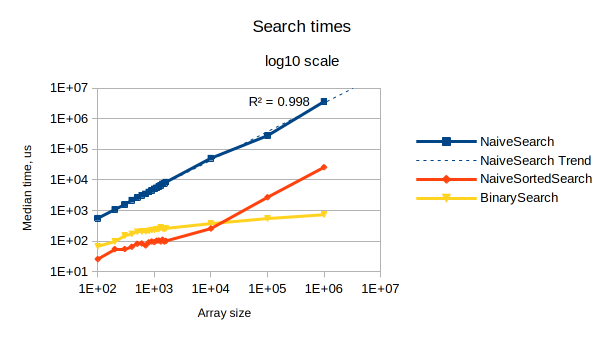
\includegraphics[width=0.9\textwidth]{logsearch.png}
        \caption{Median time vs Array size for all implementations}
        \label{fig:log-search-chart}
    \end{figure}

    \begin{figure}[H]
        \centering
        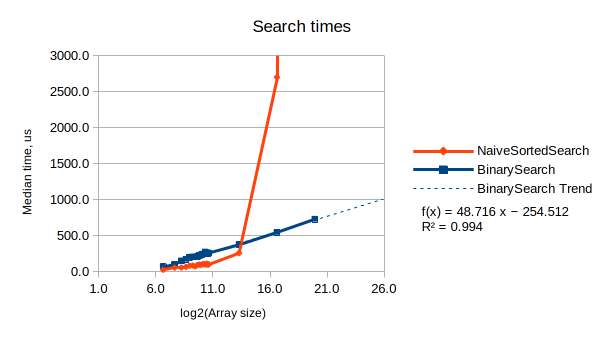
\includegraphics[width=0.9\textwidth]{log2search.png}
        \caption{Median time vs $\log_2{\left(\text{Array size}\right)}$ for the sorted naive and binary search implementations}
        \label{fig:log2-search-chart}
    \end{figure}

    \subsection*{Finding duplicates}

    Unlike in search, the naive duplicate algorithm was four orders of magnitude slower than with the binary search algorithm, while the index-based duplicate algorithm was another order of magnitude faster. The results for finding duplicates in 1M elements are given in Fig. \ref{fig:dupes-n-1M}.

    \begin{figure}[H]
        \centering
        \begin{tabular}{c|c|c|c|c}
            Function & Min, ms & Max, ms & Median, ms & Mean, ms \\
            \hline
            \hline
            \texttt{DuplicatesNaive} & 273000 & 351000 & 340000 & 315000 \\
            \hline
            \texttt{SortedDuplicatesBinary} & 44.5 & 50.3 & 44.8 & 46.3 \\
            \hline
            \texttt{SortedDuplicatesSmart} & 6.77 & 7.34 & 7.20 & 7.11 \\
        \end{tabular}
        \caption{Results for finding duplicates in 1M elements}
        \label{fig:dupes-n-1M}
    \end{figure}

    When running the duplicate finding functions across all $N$ (Fig. \ref{fig:dupes-chart}), it appears that the binary search-based algorithm is actually faster for small $N$ compared to the index-based algorithm. The naive implementation is still slower than one or the other algorithm for all $N$. The binary search algorithm is faster for small $N$ compared to the index-based algorithm because of a smaller constant factor. The index-based algorithm iterates over both arrays completely, while the binary search algorithm only iterates over the first array. At high $N$, the index-based algorithm is faster because it doesn't have to perform any searches.

    \begin{figure}[H]
        \centering
        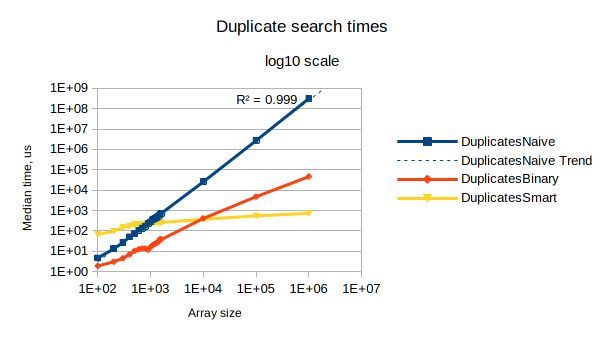
\includegraphics[width=0.9\textwidth]{dupes.png}
        \caption{Median time vs Array size for all duplicate finding implementations}
        \label{fig:dupes-chart}
    \end{figure}

    \begin{appendices}
        \section{Search benchmark implementation}
        \label{appendix:benchmark_search}

        \begin{minted}{go}
func BenchSearch(search func([]int, int) int) []SizeTime {
    sizes := []int{
        100, 200, 300, 400, 500,
        600, 700, 800, 900, 1000,
        1100, 1200, 1300, 1400,
        1500, 1600, 10000,
        100000, 1000000,
    }
    times := make([]SizeTime, 0, len(sizes))

    for _, size := range sizes {
        loop := 10000
        sortedArr := CreatedSortedIntArray(size, 1000)
        indx := keys(loop, size)

        fmt.Printf("Size: %d\n", size)

        iters := 250
        minTime := math.Inf(1)
        maxTime := math.Inf(-1)
        iterTimes := make([]float64, iters)

        for i := 0; i < iters; i++ {
            start := time.Now()

            for _, i := range indx {
                search(sortedArr, i)
            }

            elapsed := time.Since(start).Nanoseconds()
            minTime = math.Min(minTime, float64(elapsed))
            maxTime = math.Max(maxTime, float64(elapsed))
            iterTimes[i] = float64(elapsed)

            if i%100 == 0 {
                fmt.Printf(
                    "Iteration %d. Last elapsed time: %fus\n",
                    i,
                    float64(elapsed)/1000
                )
            }
        }

        times = append(times, SizeTime{
            size,
            minTime / 1000,
            maxTime / 1000,
            median(iterTimes) / 1000,
            mean(iterTimes) / 1000,
        })
    }

    return times
}
        \end{minted}

        \section{Duplicates benchmark implementation}
        \label{appendix:benchmark_duplicates}

        \begin{minted}{go}
func BenchDuplicates(findDuplicates func([]int, []int) []int) []SizeTime {
    sizes := []int{
        100, 200, 300, 400, 500,
        600, 700, 800, 900, 1000,
        1100, 1200, 1300, 1400,
        1500, 1600, 10000,
        100000, 1000000,
    }
    times := make([]SizeTime, 0, len(sizes))

    for _, size := range sizes {
        sortedArrA := CreatedSortedIntArray(size, 1000)
        sortedArrB := CreatedSortedIntArray(size, 1000)

        fmt.Printf("Size: %d\n", size)

        iters := 1000
        minTime := math.Inf(1)
        maxTime := math.Inf(-1)
        iterTimes := make([]float64, iters)

        for i := 0; i < iters; i++ {
            start := time.Now()

            findDuplicates(sortedArrA, sortedArrB)

            elapsed := time.Since(start).Nanoseconds()
            minTime = math.Min(minTime, float64(elapsed))
            maxTime = math.Max(maxTime, float64(elapsed))
            iterTimes[i] = float64(elapsed)

            if i%100 == 0 {
                fmt.Printf(
                    "Iteration %d. Last elapsed time: %fus\n",
                    i,
                    float64(elapsed)/1000
                )
            }
        }

        times = append(times, SizeTime{
            size,
            minTime / 1000,
            maxTime / 1000,
            median(iterTimes) / 1000,
            mean(iterTimes) / 1000,
        })
    }

    return times
}
        \end{minted}
    \end{appendices}

%     \section*{Stack benchmarks}

%     To benchmark the stack implementations, I did 2000 runs, each of which consisted of a 1000 iterations of N pushes and N pops (sequentially as listed). The results for each run were then written to a CSV file. Code used for benchmarking is given in appendix \ref{appendix:benchmark_code}. I benchmarked both implementations for $\forall N\in\{100, 500, 1000, 2000, 5000\}$. Unsurprisingly, the static stack outperformed the dynamic stack in all cases, as per Fig. \ref{fig:median-times}. Results for all $N$ are given in appendix \ref{appendix:results}. The speedup ratio of static over dynamic doesn't appear to change significantly over $N$ (Fig. \ref{fig:ratio}), averaging out at about $1.5$.

%     \begin{figure}[H]
%         \centering
%         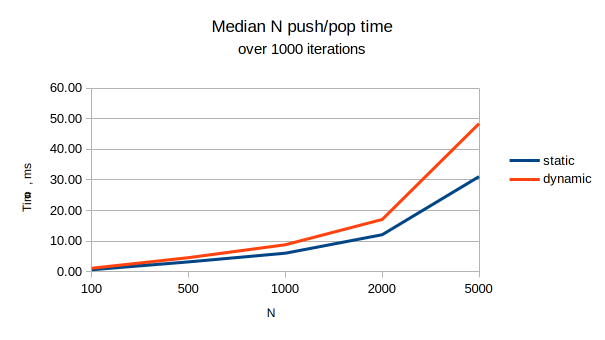
\includegraphics[width=0.9\textwidth]{median.png}
%         \caption{Median times for both implementations}
%         \label{fig:median-times}
%     \end{figure}

%     \begin{figure}[H]
%         \centering
%         \begin{tabular}{c|c}
%             N & Speedup ratio \\
%             \hline
%             \hline
%             100 & 1.8 \\
%             \hline
%             500 & 1.4 \\
%             \hline
%             1000 & 1.5 \\
%             \hline
%             2000 & 1.4 \\
%             \hline
%             5000 & 1.6 \\
%         \end{tabular}
%         \caption{$Ratio = \frac{Med(DynamicTimes)}{Med(StaticTimes)}$}
%         \label{fig:ratio}
%     \end{figure}

%     An interesting observation is that the static stack run times are more consistent than the dynamic stack run times for all $N$. This is evident in the run time histograms (Fig. \ref{fig:histo1000}). The static stack times are more consistent most likely because the stack is pre-allocated and the run time is not affected by the size of the stack. On the other hand, the dynamic stack times are more inconsistent because the stack is dynamically reallocated, thus likely more susceptible to background processes.

%     \begin{figure}[H]
%         \centering
%         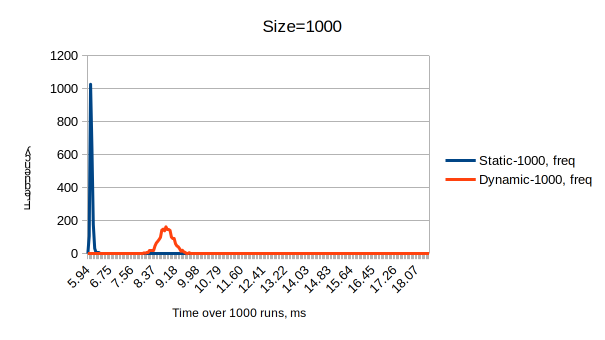
\includegraphics[width=0.9\textwidth]{size1000histo.png}
%         \caption{N=1000 run time histogram, all $N$ histograms in appendix \ref{appendix:histos}}
%         \label{fig:histo1000}
%     \end{figure}

%     \begin{appendices}
%         \section{Benchmark code}
%         \label{appendix:benchmark_code}

%         \begin{minted}{go}
% func StackBench[StackType stacks.Stack[int]](
%     tag string,
%     stack StackType,
%     runs int,
%     runIters int,
%     stackIters int
% ) {
%     outFile, err := os.Create(fmt.Sprintf("stack_%s.csv", tag))

%     if err != nil {
%         fmt.Println(err)
%         return
%     }

%     defer outFile.Close()

%     runTimes := make([]time.Duration, runs)

%     for run := 0; run < runs; run++ {
%         runStart := time.Now()

%         for iter := 0; iter < runIters; iter++ {
%             for i := 0; i < stackIters; i++ {
%                 stack.Push(i)
%             }
    
%             for i := 0; i < stackIters; i++ {
%                 stack.Pop()
%             }
%         }

%         runTimes[run] = time.Since(runStart)
%     }

%     writer := csv.NewWriter(outFile)
%     defer writer.Flush()

%     for _, time := range runTimes {
%         writer.Write([]string{fmt.Sprintf("%d", time.Microseconds())})
%     }
% }
%         \end{minted}

%         \section{Benchmark results}
%         \label{appendix:results}

%         \begin{figure}[H]
%             \centering
%             \begin{tabular}{c|c|c|c|c|c}
%                 Impl. & Min, ms & Max, ms & Mean, ms & Median, ms & Std.dev, ms \\
%                 \hline
%                 \hline
%                 Static & 0.60 & 0.91 & 0.62 & 0.62 & 0.01 \\
%                 \hline
%                 Dynamic & 0.9 & 2.7 & 1.1 & 1.1 & 0.16 \\
%             \end{tabular}
%             \caption{N=100}
%         \end{figure}
%         \begin{figure}[H]
%             \centering
%             \begin{tabular}{c|c|c|c|c|c}
%                 Impl. & Min, ms & Max, ms & Mean, ms & Median, ms & Std.dev, ms \\
%                 \hline
%                 \hline
%                 Static & 3.02 & 5.17 & 3.20 & 3.20 & 0.14 \\
%                 \hline
%                 Dynamic & 4.0 & 6.6 & 4.6 & 4.6 & 0.24 \\
%             \end{tabular}
%             \caption{Results for N=500}
%         \end{figure}
%         \begin{figure}[H]
%             \centering
%             \begin{tabular}{c|c|c|c|c|c}
%                 Impl. & Min, ms & Max, ms & Mean, ms & Median, ms & Std.dev, ms \\
%                 \hline
%                 \hline
%                 Static & 5.94 & 7.28 & 6.05 & 6.04 & 0.07 \\
%                 \hline
%                 Dynamic & 8.0 & 18.6 & 8.8 & 8.8 & 0.38 \\
%             \end{tabular}
%             \caption{N=1000}
%         \end{figure}
%         \begin{figure}[H]
%             \centering
%             \begin{tabular}{c|c|c|c|c|c}
%                 Impl. & Min, ms & Max, ms & Mean, ms & Median, ms & Std.dev, ms \\
%                 \hline
%                 \hline
%                 Static & 11.95 & 15.43 & 12.18 & 12.08 & 0.26 \\
%                 \hline
%                 Dynamic & 15.8 & 21.8 & 17.1 & 17.1 & 0.46 \\
%             \end{tabular}
%             \caption{N=2000}
%         \end{figure}
%         \begin{figure}[H]
%             \centering
%             \begin{tabular}{c|c|c|c|c|c}
%                 Impl. & Min, ms & Max, ms & Mean, ms & Median, ms & Std.dev, ms \\
%                 \hline
%                 \hline
%                 Static & 30.14 & 52.54 & 31.55 & 31.08 & 1.87 \\
%                 \hline
%                 Dynamic & 45.4 & 75.5 & 50.3 & 48.4 & 4.08 \\
%             \end{tabular}
%             \caption{N=5000}
%         \end{figure}

%         \section{Run time histograms}
%         \label{appendix:histos}

%         \begin{figure}[H]
%             \centering
%             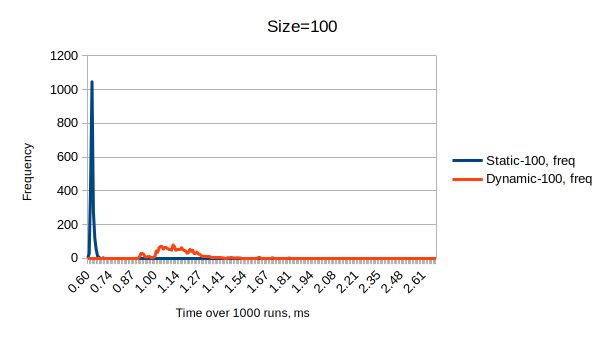
\includegraphics[width=0.9\textwidth]{size100histo.png}
%             \caption{N=100}
%         \end{figure}
%         \begin{figure}[H]
%             \centering
%             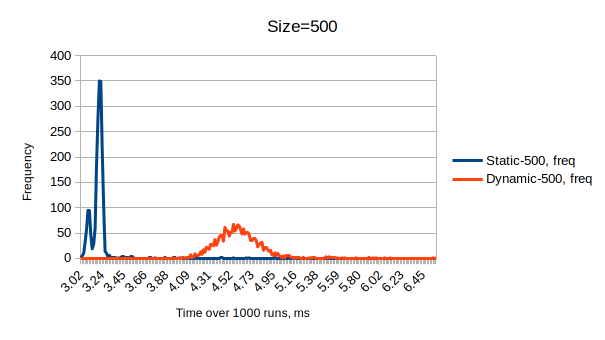
\includegraphics[width=0.9\textwidth]{size500histo.png}
%             \caption{N=500}
%         \end{figure}
%         \begin{figure}[H]
%             \centering
%             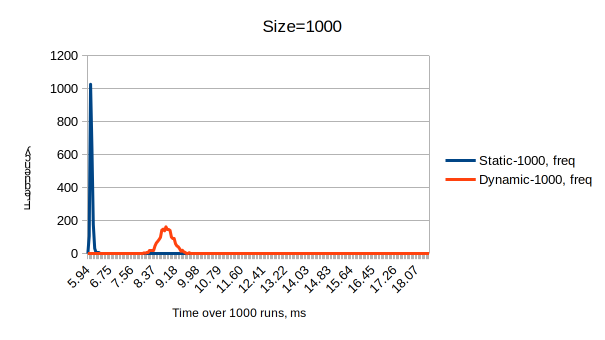
\includegraphics[width=0.9\textwidth]{size1000histo.png}
%             \caption{N=1000}
%         \end{figure}
%         \begin{figure}[H]
%             \centering
%             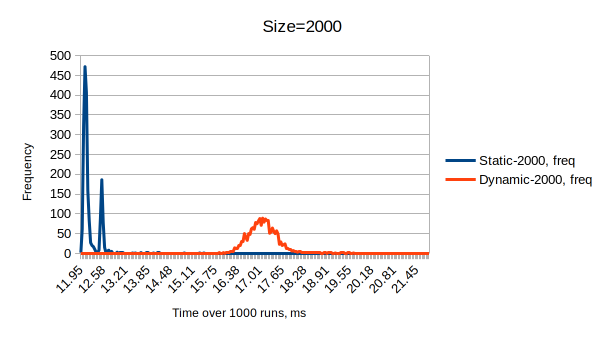
\includegraphics[width=0.9\textwidth]{size2000histo.png}
%             \caption{N=2000}
%         \end{figure}
%         \begin{figure}[H]
%             \centering
%             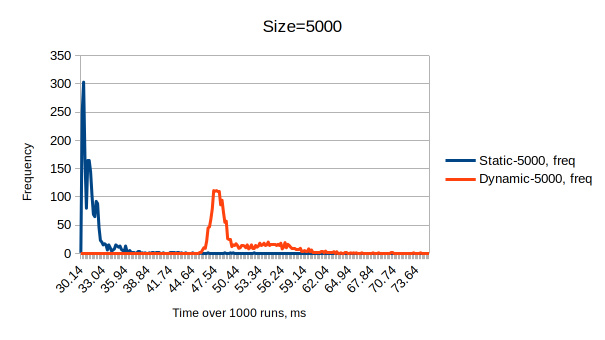
\includegraphics[width=0.9\textwidth]{size5000histo.png}
%             \caption{N=5000}
%         \end{figure}
%     \end{appendices}
\end{document}
